\documentclass{beamer}

\usepackage[english,ngerman]{babel}
\usepackage[utf8]{inputenc}
\usepackage{beamerthemeshadow}
\usepackage{amsmath}
\usepackage{listings}
\usepackage{graphicx}

\title{Recap INTRO HS16}
\subtitle{USB \& Queues}
\author[Stoffel, Walker] % (optional, for multiple authors)
{Cyrill~Stoffel \& Tobias~Walker}
\date{\today}



\setbeamertemplate{footline}
{
	\leavevmode%
	\hbox{%
		\begin{beamercolorbox}[wd=.333333\paperwidth,ht=2.25ex,dp=1ex,center]{author in head/foot}%
			\usebeamerfont{author in head/foot}\insertshortauthor
		\end{beamercolorbox}%
		\begin{beamercolorbox}[wd=.333333\paperwidth,ht=2.25ex,dp=1ex,center]{title in head/foot}%
			\usebeamerfont{title in head/foot}\insertshorttitle
		\end{beamercolorbox}%
		\begin{beamercolorbox}[wd=.333333\paperwidth,ht=2.25ex,dp=1ex,right]{date in head/foot}%
			\usebeamerfont{date in head/foot}\insertshortdate{}\hspace*{2em}
			\insertframenumber{} / \inserttotalframenumber\hspace*{2em} 
		\end{beamercolorbox}}%
	\vskip0pt%
}



%gets rid of navigation symbols
\setbeamertemplate{navigation symbols}{}


\begin{document}
	
	\frame{\titlepage}

	
	\begin{frame}
		\frametitle{Inhaltsverzeichnis}
		\tableofcontents
	\end{frame}

	\section{USB}
	\subsection{USB Allgemein}
	\begin{frame}
			\frametitle{USB Allgemein}
				\begin{figure}
					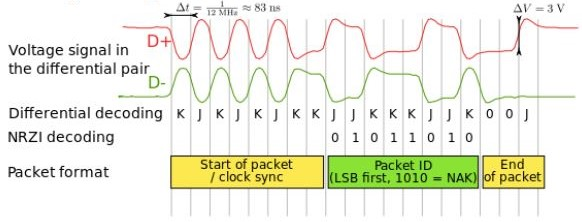
\includegraphics[width=0.7\textwidth]{usb}
				\end{figure}
			\begin{itemize}
				\item Signal $\Delta$3V
				\item Speisung 5V			
			\end{itemize}								
	\end{frame}
	
	\subsection{Frequenz}
	\begin{frame}
		\frametitle{Frequenz}
		\begin{itemize}
			\item USB: 12MHz
			\item Abtastfrequenz: 24MHz
			\item NXP Kinetis: 48MHz
		\end{itemize}
	\end{frame}

	\subsection{Aufbau}
	\begin{frame}
		\frametitle{Aufbau}
		\begin{figure}
			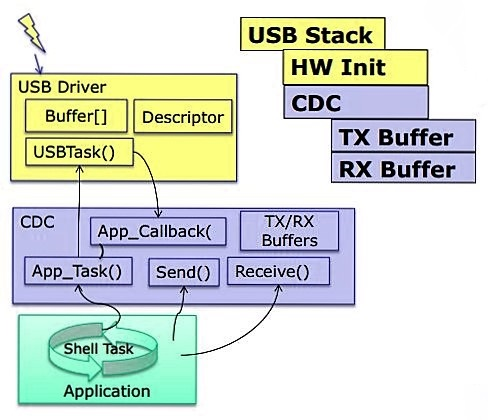
\includegraphics[width=0.8\textwidth]{stack}
		\end{figure}		
	\end{frame}


	
	\section{Queues}
	\subsection{Queues Allgemein}
	\begin{frame}
		\frametitle{Queues Allgemein}
		\begin{itemize}
			\item	Speicher wird im Heap alloziert
			\item	FIFO
			\item	LIFO
			\item	'by value'
		\end{itemize}
	\end{frame}

	\subsection{Erstellen und löschen einer Queue}
\begin{frame}[fragile]
\frametitle{Erstellen und löschen einer Queue}
\begin{lstlisting}[language = C]
xQueueHandle xQueueCreate ( 
	unsigned portBASE_TYPE uxQueueLength,
	unsigned portBASE_TYPE uxItemSize);

void vQueueDelete ( xQueueHandle xQueue );	
\end{lstlisting}
\end{frame}
	
	\subsection{Elemente entfernen}
\begin{frame}[fragile]
\frametitle{Elemente entfernen}
\begin{lstlisting}[language = C]
BaseType_t xQueueReset ( xQueueHandle xQueue );

BaseType_t xQueuePeek (
	xQueueHandle xQueue ,
	void *pvBuffer ,
	portTickType xTicksToWait );
	
BaseType_t xQueueReceive (
	xQueueHandle xQueue ,
	void *pvBuffer ,
	portTickType xTicksToWait );
\end{lstlisting}
\end{frame}

	\subsection{Elemente hinzufügen}
\begin{frame}[fragile]
\frametitle{Elemente hinzufügen}
\begin{lstlisting}[language = C]
BaseType_t xQueueSendToBack (
	xQueueHandle xQueue ,
	const void *pvItemToQueue ,
	portTickType xTicksToWait );
	
BaseType_t xQueueSendToFront (
	xQueueHandle xQueue ,
	const void *pvItemToQueue ,
	portTickType xTicksToWait );
\end{lstlisting}
\end{frame}


	\begin{frame}
		\frametitle{Frage 1}
		\begin{itemize}
			\item<1-> Mit welcher Frequenz wird das USB Modul versorgt? Welches ist die effektive Frequenz von USB?
			\item<2-> 48MHz und 12MHz
		\end{itemize}
	\end{frame}
	\begin{frame}
		\frametitle{Frage 2}
		\begin{itemize}
			\item<1-> Welchen Betrag hat die differentielle Signalspannung bei USB?
			\item<2-> $\Delta$3V	
		\end{itemize}
	\end{frame}
	\begin{frame}
		\frametitle{Frage 3}
		\begin{itemize}
			\item<1-> Das USB Device taucht unter Ports nicht auf. Woran könnte das liegen?
			\item<2-> Der clock ist falsch eingestellt oder die interrupts wurden eingeschalten bevor der USB Stack initialisiert wurde.
		\end{itemize}
	\end{frame}
	\begin{frame}
		\frametitle{Frage 4}
		\begin{itemize}
			\item<1-> Kann die Länge einer Queue dynamisch verändert werden?
 			\item<2-> Nein
		\end{itemize}
	\end{frame}
	\begin{frame}
		\frametitle{Frage 5}
		\begin{itemize}
			\item<1-> Wie werden Items in die Queue gegeben? (by reference/value)
			\item<2-> by value
		\end{itemize}
	\end{frame}

\end{document}
